\documentclass{article}
\usepackage{graphicx} % Required for inserting images
\usepackage{amsmath}
\usepackage{amssymb}
\usepackage{enumitem}
\usepackage{subfig}

\begin{document}
\begin{center}
\textbf{
{\Large HKN ECE 110 Midterm 1 Worksheet}
} 
\end{center} 
\noindent\makebox[\linewidth]{\rule{\linewidth}{0.2pt}}

\section*{Important Quantities and their Units}
\begin{enumerate}
    \item A current, $I$, flows in a wire as the graph below.\\
    What is the total charge, $\Delta Q$ that has been moved across a cross-section of that wire in the same time?\\
    \begin{figure}[!h]
        \centering
        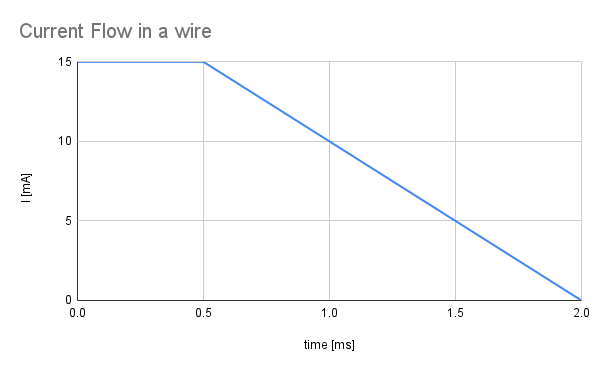
\includegraphics[width=1.1\textwidth]{figures/1.png}
    \end{figure}
    \textbf{Find the area under the curve. \\ $\Delta Q = \frac{1}{2}(2 + 0.5 ms)(15 mA) = 18.75 \mu C$}
    \item A circuit carries a charge of 12 Coulombs through a wire in 4 seconds. What is the current flowing through the circuit? \\
    \textbf{$I = \frac{Q}{t} = \frac{12 C}{4 s} = 3A$}\\
    \item A battery does 24 Joules of work to move 6 Coulombs of charge. What is the voltage of the battery?
    \\ \textbf{$V = \frac{J}{Q} = \frac{24 J}{6 C} = 4V$}
    \newpage
    
\end{enumerate}

\section*{Ohm's Law and Power}
\begin{enumerate}
    \item A circuit has a voltage of 12V and current of 2A. What is the resistance?\\\\
    \textbf{Use Ohm's Law. $R = \frac{V}{I} = \frac{12 V}{2 A} = 6 \Omega$}\\
    \item A resistor has a resistance of 5$\Omega$, and a current of 3A flows through it. What is the voltage across the resistor?\\\\
    \textbf{Use Ohm's Law. $V = IR = (3A)(5\Omega) = 15 V$}\\
    \item Three resistors with values 4$\Omega$, 6$\Omega$, and 10$\Omega$ are connected in series to a 24V battery.
    \begin{enumerate}[label=\alph*.]
        \item What is the total resistance? \\
        \textbf{The total resistance in series is the sum of the individual resistances. $R_{total} = 4\Omega + 6\Omega + 10\Omega = 20\Omega$} \\
        \item What is the current flowing through the circuit? \\
        \textbf{Use Ohm's Law. $I = \frac{V}{R} = \frac{24 V}{20 \Omega} = 1.2 A$} \\
    \end{enumerate}
    \item {Two resistors, 8$\Omega$ and 12$\Omega$, are connected in parallel. What is the equivalent resistance of the parallel combination?}\\
    \textbf{Use the formula for parallel resistors. $\frac{1}{R_{eq}} = \frac{1}{R_1} + \frac{1}{R_2} = \frac{1}{8\Omega} + \frac{1}{12\Omega} = \frac{3}{24\Omega} + \frac{2}{24\Omega} = \frac{5}{24}$}\\\\
    \textbf{$R_{eq} = \frac{24}{5} \Omega = 4.8 \Omega$}\\
    \item {A 10$\Omega$ resistor has a voltage of 20V across it.}
    \begin{enumerate}[label=\alph*.]
        \item {How much current is flowing through the resistor?}\\
        \textbf{$I = \frac{V}{R} = \frac{20 V}{10 \Omega} = 2 A$}\\
        \item {How much power is dissipated by the resistor?}\\
        \textbf{$P = IV = (2 A)(20 V) = 40 W$}\\
    \end{enumerate}
    \newpage
\end{enumerate}

\section*{Resistivity}
\begin {enumerate}
    \item A copper wire has a resistivity of $1.68*10^{-8} \Omega*m$, a length of 2m, and a cross-sectional area of $1*10^{-6} m^{2}$.\\
    \textbf{Use the formula for resistivity. \\$R = \rho \frac{L}{A} = (1.68*10^{-8} \Omega*m) \frac{2m}{1*10^{-6} m^{2}} = 0.0336 \Omega$}\\\\
    \item A 1m long aluminum wire has a resistance of 0.1$\Omega$. Given that the resistivity of aluminum is $2.82*10^{-8} \Omega*m$. What is the required diameter of the wire?\\
    \textbf{Use the formula for resistivity. \\$R = \rho \frac{L}{A} = \rho \frac{L}{\pi r^{2}}$\\
    $r = \sqrt{\frac{\rho L}{\pi R}} = \sqrt{\frac{(2.82*10^{-8} \Omega*m)(1m)}{\pi (0.1\Omega)}} = 0.0003 m$\\
    $d = 2r = 0.0006 m = 0.6 mm$}\\
\end {enumerate}

\section*{Energy and Power (Again)}
\begin{enumerate}
    \item A 100$\mu F$ capacitor is charged to 12V. How much energy is stored in the capacitor?\\
    \textbf{$E = \frac{1}{2}CV^{2} = \frac{1}{2}(100*10^{-6} F)(12 V)^{2} = 0.0072 J = 7.2 mJ$}\\\\
    \item A 60W light bulb is left on for 3 hours. How much electrical energy is consumed in joules?\\
    \textbf{$E = Pt = (60 W)(3 h)(3600 s/h) = 648000 J = 648 kJ$}\\\\
    \item A 10$\Omega$ resistor has a current of 2A flowing through it for 5 minutes. How much energy is dissipated as heat?\\
    \textbf{$E = Pt = (I^{2}R)t = (2 A)^{2}(10 \Omega)(5 min)(60 s/min) = 12000 J = 12 kJ$}\\\\
    \item Imagine we cook an egg by immersing it into water, which is boiled by an electric heater. The heater utilizes a current I = 15 A at a voltage V = 110 V for a time t = 300 s. If the change in energy of the newly cooked egg over its raw form is given by $\Delta E_{egg}$ = 72.5 kJ, what is the amount of energy wasted in the process? \\
    \textbf{$E = Pt = IVt = (15 A)(110 V)(300 s) = 495000 J = 495 kJ$}\\\\
    \textbf{$E_{wasted} = E - \Delta E_{egg} = 495 kJ - 72.5 kJ = 422.5 kJ$}
\end{enumerate}



\end{document}

